\section{Results}

The rocket RORO I flew twice. The first flight was a test flight in Switzerland and the second flight was the competition flight at Spaceport America Cup.

On board of the rocket there were an Inertial Measurement Unit (IMU) and a barometer that logged data to an SD card.
This data has been analyzed for both of the flights.

\subsection{Rocket Test Flight}
\label{subsection:flightTests}

The test flight was performed in Kaltbrunn, Switzerland to a target apogee of 565m using an Aerotech K1275 motor and a lift-off mass of 18.3 kg. The apogee was limited to 600m due to proximity to buildings.

The rocket flight was successful, to an apogee of 502m, with two anomalies:
\begin{itemize}
    \item The main parachute opened at apogee instead of at 200m above ground
    \item The rocket oscillated at a high angle of attack
\end{itemize}

The main chute opening cause has been identified from the high quality video of the optical tracking done by ETHZ.
In conclusion, the parachute opening at apogee has been caused from the shock of the separated rocket stretching out the shock cord to the drogue parachute, where also the main chute bag was attached.
This shock pulled the main chute cords out of the bag, which then pulled out the entire main chute.

This design problem has been fixed by securing the main chute cords in the bag until the chute is released.

The second anomaly, the oscillation and high angle of attack, required an analysis of the IMU data as the cause of the high angle of attack could not be identified simply from video footage.

\subsubsection{IMU Data Analysis}

In the following, the z-axis is the roll axis and points down along the rocket and the x and y-axes are pitch and yaw respectively.

The IMU on board the rocket was an MPU-6000 MEMS 3-axis gyroscope and 3-axis accelerometer from InvenSense.

The gyroscope measures angular rate which has to be integrated to obtain the attitude of the rocket.
To reduce attitude drift due to high zero-rate bias of these MEMS gyroscopes, the bias was estimated by taking the average output while the rocket was on the launch rail from 30 seconds before lift-off to 5 seconds before lift-off.
This should give a reasonably precise attitude for the approximately 10 seconds to apogee.

The accelerometer bias could not be calibrated on the launch pad, as the precise inclination of the launch-rail was not known.
Therefore the accelerometer was calibrated after the flight for scale and bias by sequentially placing the IMU on each of the six faces up.
The bias for an axis is obtained by taking the mean between the averaged positive one $g$ acceleration and averaged negative one $g$ acceleration.
The scale for the axis is obtained by taking the half of the difference between the positive and negative one $g$ acceleration.
\begin{align}
    bias_i &= \frac{a^{+g}_i + a^{-g}_i}{2} \\
    scale_i &= \frac{a^{+g}_i - a^{-g}_i}{2g}
\end{align}


After sensor calibration, the first step was to integrate the angular rate to obtain the attitude of the rocket.
The attitude throughout the flight was visualized in 3D.
In the animation the tilting and subsequent oscillation of the rocket was well visible, but the source of the disturbance was not evident.


The next step was to correct the calibrated IMU accelerations for centripetal and tangential accelerations due to angular rate and angular acceleration, as the IMU is not placed at the center of mass. This gives us the acceleration at the center of mass:
\begin{equation}
    \bm{a}_{CM} = \bm{a}_{IMU} - \bm{a}_{tangential} - \bm{a}_{centripedal}
\end{equation}
\begin{equation}
\begin{split}
    \bm{a}_{tangential} &= \bm{\dot\omega} \times \bm{r}_{IMU} \\
    \bm{a}_{centripedal} &= - |\bm{\omega}_{tangential}|^2  \bm{r}_{IMU} \\
    \bm{\omega}_{tangential} &= \bm{\omega} - \frac{\bm{\omega} \cdot \bm{r}_{IMU}}{\bm{r}_{IMU}^2}\bm{r}_{IMU}
\end{split}
\end{equation}
where $\bm{r_{IMU}}$ is the position of the IMU with respect to the center of mass

The center of mass location is obtained from the Solidworks CAD (which was experimentally verified for the lift-off configuration) and is linearly interpolated from lift-off configuration to burn-out configuration for the time of the motor burn. This is good enough, as the motor burn curve is quite constant.

This acceleration at the center of mass was then used to compute the side-forces acting on the rocket using the known mass. Again the mass is interpolated during the burn as for the center of mass.

With the assumption that the side forces are aerodynamic, they should act at the center of pressure, which can be analytically determined.
This results in a moment which was calculated using \ref{eq:m_aero}.
\begin{equation}
\label{eq:m_aero}
\begin{split}
    M^{aero}_x &= (z_{CP} - z_{CM}) (-F_y) \\
    M^{aero}_y &= (z_{CP} - z_{CM}) F_x \\
\end{split}
\end{equation}

This aerodynamic moment was then compared with the actual moment that was acting on the rocket.
The actual moment was obtained from the angular rates and the inertia by use of the Euler equations for rigid body dynamics. For an equal pitch and yaw inertia these equations are:
\begin{equation}
\begin{split}
    M_x &= I_{xy} \dot\omega_x + (I_z-I_{xy}) \omega_y \omega_z \\
    M_y &= I_{xy} \dot\omega_y + (I_{xy}-I_z) \omega_z \omega_x \\
    M_z &= I_{z} \dot\omega_z
\end{split}
\end{equation}


The comparison between aerodynamic model based moments and actual moments is show in figure \ref{fig:test_flight_graph}.
\begin{figure}[h!]
    \centering
        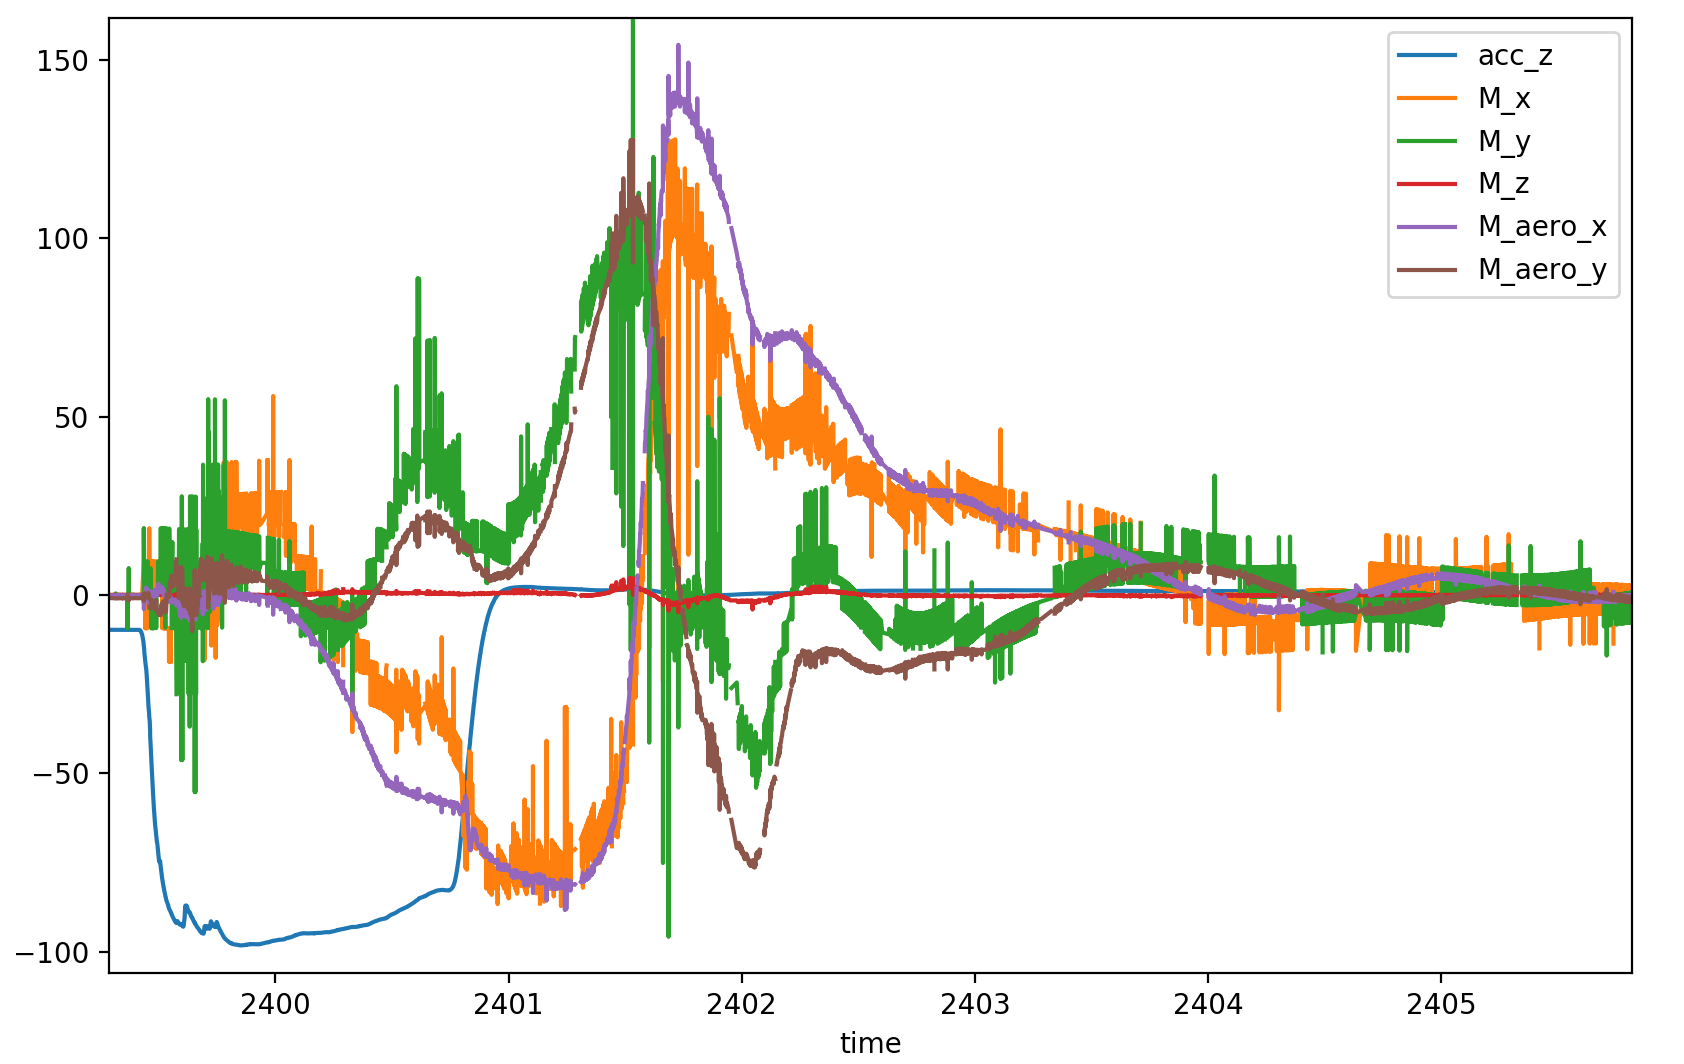
\includegraphics[width=0.5\textwidth]{img/test_flight_graph.png}
        \caption{Comparison of predicted aerodynamic moments (M_aero_xy) and actual moments (M_xyz). The duration of the motor burn is clearly visible in the z acceleration.}
        \label{fig:test_flight_graph}
 \end{figure}

The following observations are made:
\begin{itemize}
\item The moment after burnout and reduction of oscillations to reasonable angles of attack matches well with aerodynamic prediction. This validates our analytic center of pressure determination.
\item The moment after burnout but at high angles of attack is slightly lower than predicted by the aerodynamic model. This is to be expected, as the model does not include the cylindrical body lift which increases with angle of attack, moving the center of pressure forward. A more forward center of pressure would result in the smaller moments that were seen at high angle of attack.
\item During the burn there is a permanent, about 20Nm mismatch between the aerodynamic prediction and the actual moments. After burnout this difference vanishes.
\end{itemize}

The first two points validated the aerodynamic model.
They also showed that there was no torque acting on the rocket other the expected aerodynamic restoring torques at non-zero angle of attack.

The third point gives an important clue to the origin of the disturbance. For the duration of the motor burn, there was a moment that is not of aerodynamic origin.
The best explanation is that this moment was caused by a misalignment of the motor thrust with respect to the center of gravity.

A side accelerometer sensitivity to forward acceleration can be ruled out, as the side acceleration is around zero while accelerating on the launch rail.
The same applies for the gyroscope that is close to zero until leaving the launch rail.

There are several possible causes for the thrust misalignment.
\begin{itemize}
    \item The center of gravity is not centered in the rocket
    \item The rocket motor is not centered in the rocket
    \item The rocket motor was not aligned with the rocket body
    \item The rocket body bent under load which place the CG out of the line of thrust
    \item The rocket motor was aligned, but produced a side-thrust.
\end{itemize}

With the K1275 motor the thrust misalignment which created a torque of 20Nm would correspond to an off-center CG respectively motor centering of 15mm or a motor misalignment of 0.79 degree.
Careful inspection and measuring of the rocket ruled out all the above mentioned possible causes except for the last one. Unfortunately we did not keep the nozzle, which is a consumable of the COTS motor assembly. Therefore it is impossible to check if any asymmetries are visible in the erosion of the nozzle.

\subsubsection{Test Flight Analysis Conclusion}

The high angle of attack during the test flight was caused by a thrust misalignment. The most probable explanation for the thrust misalignment seems to be a defect in the Aerotech K1275 COTS motor.

The reason for the lower apogee than the predicted one is due to the higher drag of the rocket flying at an angle of attack. Therefore it is important to dampen oscillations quickly so that the rocket minimizes the time where it is at a high angle of attack after a disturbance.

As a result of the conclusion of the IMU data analysis we were faced with a design trade-off.
We wanted to increase the damping of oscillations and at the same time increase the corrective force of the fins, to be able to withstand a potential thrust misalignment of a motor with more thrust that would be used for the competition flight.
Unfortunately with an increase of corrective force of the fins, the damping ratio decreases, which increases the time to dampen oscillations.

As the exact source of the thrust misalignment could not be identified, we decided to sacrifice some of the damping and increase the corrective force of the fins to the maximum that was within the guidelines of the competition.
For this, we increased the surface of span of the fins by 30\%. The resulting corrective force for a certain angle of attack was about doubled and the damping ratio went from 0.13 to 0.083.
We estimated that this would give us enough safety to withstand a similar thrust misalignment angle with the stronger motor used at the competition.

\subsection{Rocket Competition Flight}


\subsection{Glider Test Flights}

TODO picture of glider and big wing

\subsection{Glider Competition Flight}

TODO analysis of the landing site

